\scanpage{25}
\noindent\handwritten{SGA 4 $\overline{\text{\uline{IX}}}$\quad p. 42}\hfill
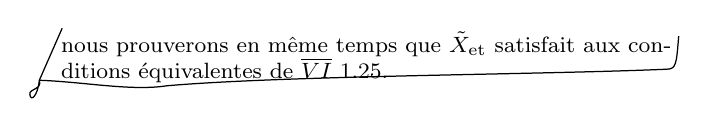
\begin{tikzpicture}[baseline=(topnote.north),x=1cm,y=1cm]
\node[anchor=north west,inner sep=0pt,text width=7.8cm,align=left,font=\footnotesize] (topnote) at (.25,0) {\handwritten{nous prouverons en même temps que $\tilde{X}_{\mathrm{et}}$ satisfait aux conditions équivalentes de $\overline{\text{\uline{VI}}}$ 1.25.}};
\draw[line width=.45pt] (.27,.04)--(-.02,-.62) .. controls (-.04,-.82) and (-.13,-.90) .. (-.14,-.80) .. controls (-.16,-.73) and (.02,-.74) .. (-.02,-.62);
\draw[line width=.45pt] (-.02,-.62) .. controls (.55,-.64) and (1.15,-.76) .. (1.60,-.69) .. controls (3.1,-.56) and (6.3,-.55) .. (7.94,-.48) .. controls (8.07,-.48) and (8.07,-.42) .. (8.10,-.06);
\end{tikzpicture}

\handwritten{(*) (Note pour la page 8.) Prouvons que la notion de constructibilité 2.3 pour un faisceau d'ensembles $F$ coïncide avec celle de $\overline{\text{\uline{VI}}}$ 1.9.3. \deleted{Soit} La \deleted{en effet $C$ le \unsure{cas}}\inserted{question étant} locale sur $X$, on peut supposer $X$ affine \inserted{donc ``cohérent'', i.e.} quasi-compact et quasi-séparé. \deleted{Soit $C$ la catégorie \unsure{Soit $C(C')$ le sous-caté|Soit $(C')$ le sous-caté}} \deleted{Je faut alors prouver que $F$ est constructible} Soit $C$ (resp. $C'$) la sous-catégorie \deleted{\unsure{quasi|pleine}}\inserted{strictement} pleine de $\tilde{X}_{\text{ét}}$ formée des $F$ constructibles au sens de 2.3, \deleted{\illegible{1}} \inserted{(resp. au sens de $\overline{\text{\uline{VI}}}$ 1.9.3), il} faut prouver \deleted{que $C$ s'identifie à la catégorie des objets \uline{cohérents} de} \deleted{\unsure{$\tilde{X}_{\mathrm{et}}$}} que $C=C'$;}

% The entire following argument is cancelled by the reproduced long strokes.
% Only the earlier local cancellations additionally use \deleted.
\noindent\begin{tikzpicture}[x=.008cm,y=-.008cm,font=\fontsize{8}{9}\selectfont]
\node[anchor=base west,inner sep=0pt,rotate=6] at (355,118) {\handwritten{En vertu de $\overline{\text{\uline{VII}}}$ 5.6 a), \deleted{l'objet final $X$ de} $\tilde{X}_{\mathrm{et}}$}};
\node[anchor=base west,inner sep=0pt,rotate=6] at (18,223) {\handwritten{\deleted{est cohérent, donc} $C'$ est formé des objets \uline{cohérents} \deleted{\unsure{($\overline{\text{\uline{VI}}}$)|$\overline{\text{\uline{VI}}}$}} de $\tilde{X}_{\mathrm{et}}$ (2.5).}};
\node[anchor=base west,inner sep=0pt,rotate=6] at (18,273) {\handwritten{En vertu de $\overline{\text{\uline{VI}}}$ 1.24, \deleted{\unsure{et}} et compte tenu du fait que $C$ est génératrice}};
\node[anchor=base west,inner sep=0pt,rotate=6] at (18,345) {\handwritten{dans $\tilde{X}_{\mathrm{et}}$ (2.7.2) et stable par limites inductives finies (2.\unsure{6|8} (i)),}};
\node[anchor=base west,inner sep=0pt,rotate=6] at (18,403) {\handwritten{il suffit de prouver que $C\subset C'$, Mais il résulte de 2.7 que tout}};
\node[anchor=base west,inner sep=0pt,rotate=6] at (18,475) {\handwritten{$F\in\mathrm{ob}\,C$ est \uline{quasi-compact}, puisque un \deleted{\unsure{$G\in\mathrm{ob}\,X_{\mathrm{et}}$} \unsure{représentable par un}}}};
\node[anchor=base west,inner sep=0pt,rotate=6] at (933,356) {\handwritten{\inserted{$G\in X_{\text{ét}}$}}};
\node[anchor=base west,inner sep=0pt,rotate=6] at (18,540) {\handwritten{\deleted{schéma $\unsure{X'|X}$} qui est quasi-compact et quasi-séparé est quasi-compact}};
\node[anchor=base west,inner sep=0pt,rotate=6] at (18,602) {\handwritten{comme objet de $\tilde{X}_{\mathrm{et}}$ \deleted{(5.6.1)} ($\overline{\text{\uline{VII}}}$ 5.6.1). \deleted{D'autre part pour}}};
\node[anchor=base west,inner sep=0pt,rotate=6] at (18,678) {\handwritten{\deleted{\unsure{voir que} $\unsure{F|F'}\unsure{\in|\to}\unsure{\mathrm{ob}\,X'|X'}$ la diagonale $F\longrightarrow\unsure{F\mathbin{\times}_{X}F|F\mathbin{\times}F}$ est quasi-compacte,}}};
\node[anchor=base west,inner sep=0pt,rotate=6] at (18,738) {\handwritten{\deleted{il suffit de voir que \unsure{pour tout} \illegible{2} \unsure{et que}\illegible{2}}}};
\node[anchor=base west,inner sep=0pt,rotate=6] at (18,803) {\handwritten{\deleted{\unsure{ce fait que $C$ est stable par produits}}}};
\node[anchor=base west,inner sep=0pt,rotate=6] at (535,713) {\handwritten{Comme $C$ est stable par \deleted{limites projectives}\inserted{produits}}};
\node[anchor=base west,inner sep=0pt,rotate=6] at (18,863) {\handwritten{finis, l'inclusion $C\subset C'$ est donc un cas particulier de 2.1.}};
\node[anchor=base west,inner sep=0pt,rotate=6] at (125,814) {\handwritten{\inserted{(2.6 (ii))}}};
% Stepped enclosing strokes, in the geometry observed on the source.
\draw[line width=.65pt] (330,62)--(325,188)--(22,218)--(36,865)--(1380,729) .. controls (1400,722) and (1410,683) .. (1427,648);
\draw[line width=.6pt] (22,455)--(765,370)--(724,386)--(724,311)--(1375,267) .. controls (1400,290) and (1420,332) .. (1430,365);
% Inner cross-hatched cancellation: a right-hand start and a long sloping strip.
\draw[line width=.6pt] (930,493)--(1388,454)--(1400,514);
\draw[line width=.6pt] (22,650)--(1396,538) .. controls (1404,552) and (1404,584) .. (1388,585) .. controls (1378,576) and (1399,564) .. (1396,582)--(730,637)--(731,657)--(20,738)--(26,800)--(485,760)--(488,690);
\draw[line width=.5pt] (30,652)--(100,727) (34,731)--(94,650);
\draw[line width=.5pt] (113,644)--(183,718) (117,721)--(179,640);
\draw[line width=.5pt] (200,636)--(269,708) (204,712)--(264,631);
\draw[line width=.5pt] (290,629)--(354,699) (292,704)--(350,623);
\draw[line width=.5pt] (380,619)--(446,692) (382,697)--(442,615);
\draw[line width=.5pt] (470,611)--(537,682) (472,688)--(533,605);
\draw[line width=.5pt] (560,603)--(627,676) (562,680)--(623,598);
\draw[line width=.5pt] (650,594)--(717,665) (652,672)--(713,588);
\draw[line width=.5pt] (949,491)--(1020,561) (951,564)--(1016,482);
\draw[line width=.5pt] (1032,483)--(1103,553) (1034,557)--(1099,475);
\draw[line width=.5pt] (1116,475)--(1188,546) (1118,549)--(1184,466);
\draw[line width=.5pt] (1200,467)--(1272,538) (1202,541)--(1268,458);
\draw[line width=.5pt] (1283,459)--(1377,529) (1285,533)--(1349,450);
\draw[line width=.5pt] (76,795)--(451,710) (170,796)--(475,730);
% Long oblique cancellation strokes across the complete abandoned proof.
\draw[line width=.65pt] (27,217)--(374,787);
\draw[line width=.65pt] (291,190)--(673,800);
\draw[line width=.65pt] (409,51)--(915,780);
\draw[line width=.65pt] (696,46)--(1185,740);
\draw[line width=.65pt] (932,26)--(1395,663);
\draw[line width=.65pt] (1195,23)--(1435,367);
\draw[line width=.65pt] (1340,8)--(1430,106);
\end{tikzpicture}
\reversemarginpar
\margin{\begin{tikzpicture}[x=1cm,y=1cm]
\node[rotate=32,align=left,inner sep=0pt,font=\scriptsize] at (.88,.65) {\handwritten{\deleted{\unsure{pourquoi|pour}}\\\handwritten{\deleted{par exemple}}}};
\draw[line width=.45pt,rotate around={32:(.88,.65)}] (.88,.65) ellipse (1.02 and .55);
\draw[line width=.5pt] (.08,.76)--(1.10,-.06) (.41,1.12)--(1.37,.25) (.92,1.29)--(1.65,.58) .. controls (1.75,.36) and (1.79,.73) .. (1.76,.97);
\end{tikzpicture}}
\normalmarginpar

\handwritten{En vertu de $\overline{\text{\uline{VI}}}$ 2.9, b), il suffit de voir que $C$ est stable pour limites inductives finies et limites projectives finies, qu'elle est génératrice, et formée d'objets quasi-compacts. \deleted{\illegible{1}} Compte tenu de 2.6 (i) et (2.7.2), il reste à prouver que tout $F\in\mathrm{ob}\,C$ est quasi-compact. Or \deleted{cela résulte}\inserted{en vertu de} de 2.7 \deleted{et $\overline{\text{\uline{VI}}}$ 1.3}, \deleted{puisque}\inserted{il existe} un $G\in\mathrm{ob}\,X_{\mathrm{et}}$ \deleted{et} qui est \inserted{un schéma} quasi-compact et quasi-séparé \deleted{et est} et un épimorphisme $G\longrightarrow F$. Or $G$ \deleted{\unsure{comme on}} est un objet quasi-compact de $\tilde{X}_{\mathrm{et}}$ ($\overline{\text{\uline{VII}}}$ 5.6.1), donc $F$ est quasi-compact ($\overline{\text{\uline{VI}}}$ 1.3), qfd.}

\handwritten{Bien entendu, il y aurait \inserted{eu} lieu de refondre les §§ 1,2 du présent exposé, \inserted{notamment} en les rattachant \inserted{\deleted{\unsure{explicitement}}} aux notions générales de \deleted{l'exposé} finitude de $\overline{\text{\uline{VI}}}$. Nous laissons ce soin \deleted{\unsure{complémentaire}} de rédaction aux générations futures.}
% archive sheet number: 24
